Most numerical and experimental studies into Rayleigh-B\'enard Convection (RBC) assume that momentum and heat transport are done by turbulent mixing and advection, and that molecular diffusivities can be neglected. This allows RBC to be studied with the the classical Oberbeck-Boussinesq (OB) assumption, where fluid material properties are constant everywhere except in the buoyant force term. \cite{Glatzmaier2014} 

\begin{figure}[H]
	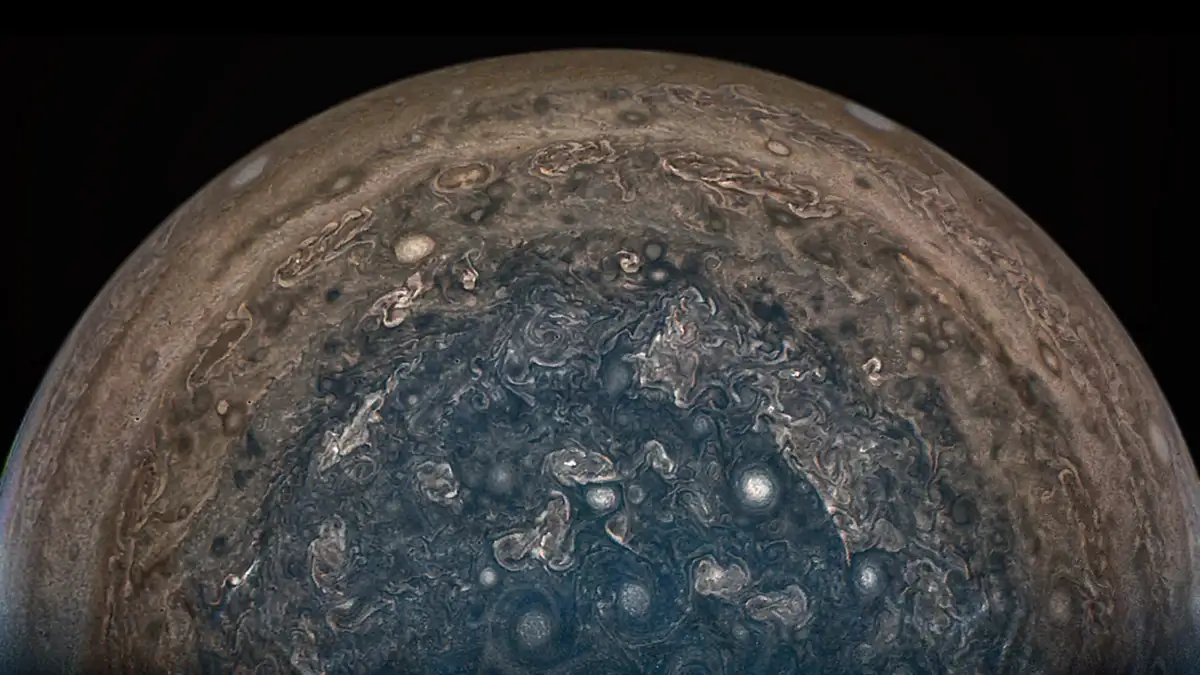
\includegraphics[width=0.45\textwidth]{img/juno-jupitersp.png}
\end{figure}

The interior of gas giants comprises of multiple layers of rapidly rotating fluids with height and temperature dependent material properties. Using Jovian-inspired material properties with non-Oberbeck-Boussinesq (NOB) Rayleigh-B\'enard equations, we want to investigate the effect of temperature-dependent viscosity, $\nu$ and thermal diffusivity, $\kappa$ on the flow morphology of rapidly-rotating RBC.









